\documentclass{beamer}


\mode<presentation>
{
  \usetheme{Goettingen}
  \usecolortheme{beaver}
  %\setbeamercovered{transparent}
}


\usepackage[danish]{babel}
\usepackage{times}
\usepackage[T1]{fontenc}
\usepackage[absolute,overlay]{textpos}
% Or whatever. Note that the encoding and the font should match. If T1
% does not look nice, try deleting the line with the fontenc.


\title{Crowd modelling}

\subtitle
{Mathematics problem formulation seminar} % (optional)

\author{Toke Høiland-Jørgensen, Mikkel Hartmann, Dan Albrechtsen, Malik 
Thrane, Troels Christensen, Wence Xiao}

\date{6th of October 2010}

%\subject{}
% This is only inserted into the PDF information catalog. Can be left
% out. 


% If you have a file called "university-logo-filename.xxx", where xxx
% is a graphic format that can be processed by latex or pdflatex,
% resp., then you can add a logo as follows:
%\logo{\pgfuseimage{university-logo}}


% Delete this, if you do not want the table of contents to pop up at
% the beginning of each subsection:
%\AtBeginSubsection[]
%{
  %\begin{frame}<beamer>{Outline}
    %\tableofcontents[currentsection,currentsubsection]
  %\end{frame}
%}


% If you wish to uncover everything in a step-wise fashion, uncomment
% the following command: 

%\beamerdefaultoverlayspecification{<+->}

\begin{document}

\begin{frame}
  \titlepage
\end{frame}


\section{Introduction}
\begin{frame}{Why model crowds?}
    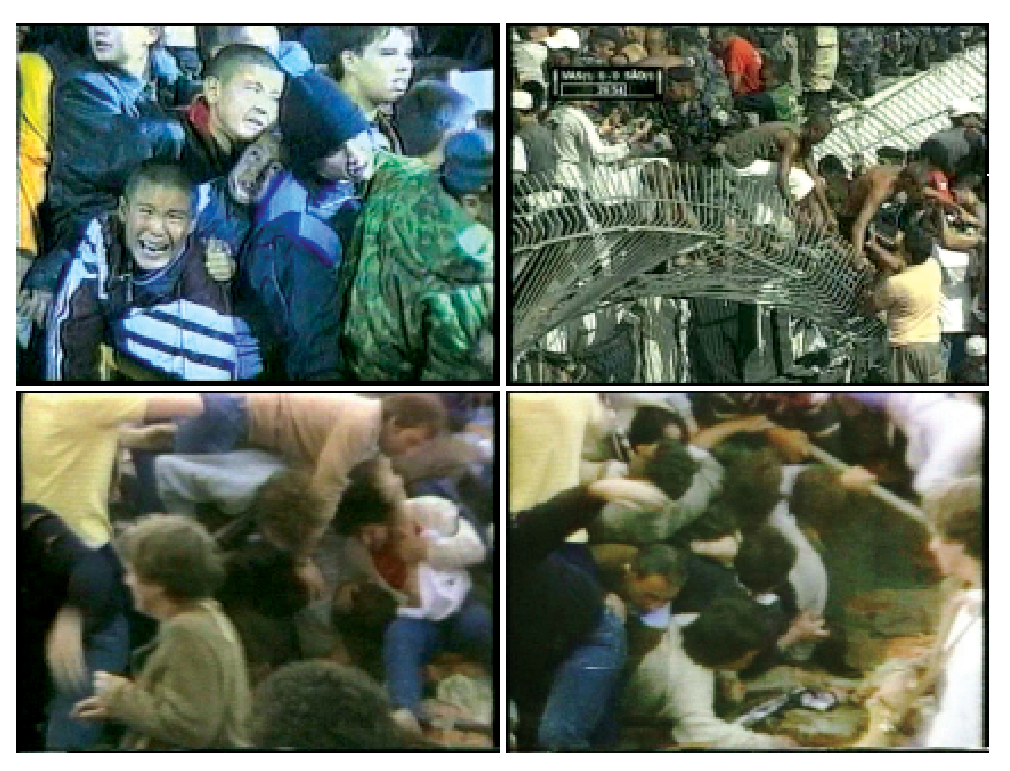
\includegraphics[width=\textwidth]{page-pictures-crop.pdf}
\end{frame}


\begin{frame}{What is crowd modelling?}
    \begin{itemize}
    	\item The purpose of crowd modelling.
        \item Not obvious how crowds move around.
        \item Hard to do experiments (esp. of panics!)
        \item Potential for better building design, optimization, avoidance of 
            injuries.
    \end{itemize}
\end{frame}

\begin{frame}{Several approaches}
    \begin{itemize}
    	\item Macro vs. Micro
        \item Rule-based models
        \item Cellular automata
        \item Particle system and dynamics
        \item Hybrids models
        \item \textbf{Social forces model}
    \end{itemize}
\end{frame}

\begin{frame}{Why is the social forces model interesting?}
    \begin{itemize}
        \item Agent-based model. Results about the system from description of 
            individual agents.
        \item ``Makes sense'' in everyday terms.
    \end{itemize}
\end{frame}

\section{Problem formulation}
\begin{frame}{Our problem formulation}
    \begin{quote}
        Can we give a meaningful characteristic for how a crowd behaves by 
        making a simulation of a social force mathematical model?
    \end{quote}
    \begin{itemize}
        \item Which meaningful characteristics are there for crowd behaviour?
            \begin{itemize}
                \item What can we say about these characteristics (origin 
                    etc.)?
            \end{itemize}
        \item How do model parameters affect the characteristics?
    \end{itemize}
\end{frame}

\begin{frame}{Why is the project exemplary?}
    \begin{itemize}
        \item Mathematical theory applied to an area outside math itself.
        \item Has non-trivial math in it.
        \item Not completely new field.
        \item Instance of a type of model used in many areas (agent-based 
            simulation).
    \end{itemize}
\end{frame}


\section{Our approach to the project}
\begin{frame}{How will we solve our problem?}
    \begin{itemize}
            \item Look at one or more social force models and determine which 
                characteristics are used for describing crowds.
            \item Make a \textbf{computer simulation} of the model(s) and try 
                to say something about the identified characteristics from 
                this simulation.
            \item Try varying the parameters of the model and see how this 
                affects the characteristics.
            \item Assess the characteristics; are they meaningful?
    \end{itemize}
\end{frame}

\begin{frame}{What are we \emph{not} going to do?}
    \begin{itemize}
        \item Empirical study (looking at an actual crowd).
        \item A model describing a crowd collectively (e.g. by density etc.)
        \item Other types of models (Non-social force. Rule-based, cellular 
            automata)
    \end{itemize}
\end{frame}



\end{document}
